\begin{section}{Archimedes' Principle}
    Archimedes' principle can be found in several general physics textbooks.The definition
    given in \cite{RESNICK} is considered and it states: 
    
    \textit{``A body wholly or partially immersed in a fluid will be buoyed up by a 
            force equal to the weight of the fluid that the body displaces"}
    
    Let's consider an impermeable body of volume $V$ and and mass $m$ with an uniform and constant 
    mass density $\rho_0$ inmersed in a fluid of density $\rho_{\omega}$ as shown bellow.\\
    
    \begin{center}
        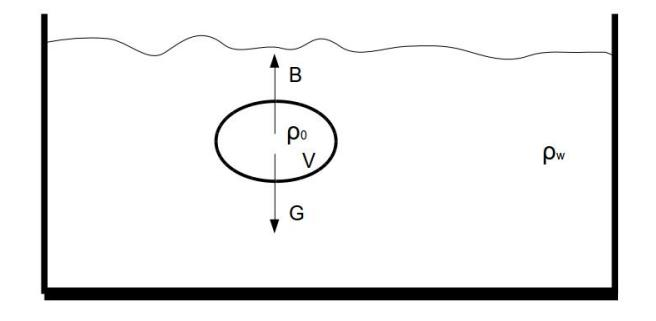
\includegraphics[scale=0.4]{./pics/buoyancy.jpg}
    \end{center}
    
    Acording to Archimedes' principle and Newton's second law if the force buoying up the 
    body is denoted by $B$ and the weight is $G$, then the the dynamics of this body is 
    described by the next equation,
    
    \begin{equation}
        \label{dynamis_00}
        B - G = m a,
    \end{equation}    
    the phenomenology described in the last session is fully contained in this formula. 
    Indeed, first if force of gravity is smaller than the force of buoyancy then 
    acceleration is positive and the body is pulled up. The force of gravity may be
    equal to the force of buoyancy and then the body remains at rest, inmersed. Finally if
    the force of gravity is bigger than the force of buoyancy then the body begins to 
    dip down until reaching the botton.
    
    Actually there is more information in equation (\ref{dynamis_00}). Archimedes principle 
    for the buoyancy force $B$ and the properties of this body lead to,
    
    \begin{eqnarray}
        m &=& \rho_0 V
        \nonumber \\
        \label{model_relations}
        B &=& \rho_{\omega} V g \\
        G &=& \rho_0 V g,
        \nonumber
    \end{eqnarray}
    doing some algebra on equation (\ref{dynamis_00}), relations (\ref{model_relations}) lead
    to a formula for accelerarion which depends only on densities; this formula is given by,
    
    \begin{equation}
        \label{dynamis_01}
        a = \left(\frac{\rho_{\omega} - \rho_0}{\rho_0} \right)g.
    \end{equation}
    
    Taking a look to this relation, the physics behind it is again the same discussed previously,
    just with the most accurate result that motion depends on densities. Indeed, first if body's 
    density is smaller than fluid's density then acceleration is positive and the body is pulled 
    up until it is partially inmersed in the fluid. Densities may be equal, then forces are 
    balanced and the body remains at rest, inmersed. Finally if body's density is bigger than 
    fluid's density then the body weight is bigger than buoyancy force and the body goes down until 
    it reaches the botton.
    
    Densities must be handle with care; thats why impermeability was requested since if the body
    allows the fluid to go inside without changing its shape, its density in average will be 
    bigger. Uniform and constant density avoids the cases in which there is one or more cavities 
    inside the body, in this case the buoyancy does not change but this fact inplies $ m \neq \rho_0 V$.
    
    What will happen if instead the object in the picture above we consider fish, indeed, fish!!. 
\end{section}
